\documentclass[12pt]{article}
\pagestyle{plain}
\usepackage[paper=letterpaper,
        left=1in,
        right=1in,
        top=1in,
        bottom=1in] {geometry}
        
\usepackage[parfill]{parskip}
\usepackage{amsmath,amssymb}
\usepackage{tikz}
\usepackage{pgf}
\usepackage{tikz}
\usetikzlibrary{positioning,arrows,automata}
\usepackage[latin1]{inputenc}

\begin{document}
\begin{center}
{\large CS 291}\\
Homework 7
\end{center}

\begin{flushright}
Jingbo Wang\\
jw6347
\end{flushright}

\textbf{Section 11.1, Exercise 2.b}  Find a regular expression to describe each of the following languages.\\
 $\{aa, ab, ac\}$\\

\textbf{Answer:}

\begin{center}
\begin{eqnarray*}
\{aa, ab, ac\} 
& = & \{a\} \{a, b, c\} \\
& = & a(a+b+c)\\
\end{eqnarray*}
\end{center}

\textbf{Section 11.1, Exercise 2.d}  Find a regular expression to describe each of the following languages.\\
  $\{a, aaa, aaaaa, ... , a^{2n+1}, . . . \}$\\

\textbf{Answer:}

\begin{center}
\begin{eqnarray*}
\{a, aaa, aaaaa, ... , a^{2n+1}, . . . \} 
& = & \{a\} \{\Lambda, aa, aaaa, ... , a^{2n}, ...\} \\
& = & \{a\} \{\Lambda, aa, (aa)^2, ... , (aa)^n, ...\}\\
& = & \{a\} \{aa\}^*\\
& = & a(aa)^*\\
\end{eqnarray*}
\end{center}

\textbf{Section 11.1, Exercise 2.e}  Find a regular expression to describe each of the following languages.\\
  $\{\Lambda, a, abb, abbbb, ... , ab^{2n}, . . . \}$\\

\textbf{Answer:}

\begin{center}
\begin{eqnarray*}
\{\Lambda, a, abb, abbbb, ... , ab^{2n}, . . . \} 
& = & \{\Lambda\} + \{a\} \{\Lambda, bb, ... , b^{2n}, ...\}\\
& = & \{\Lambda\} + \{a\} \{\Lambda, bb, ... , (bb)^n, ...\}\\
& = & \{\Lambda\} + \{a\} \{bb\}^*\\
& = & \Lambda + a(bb)^*\\
\end{eqnarray*}
\end{center}

\textbf{Section 11.1, Exercise 4.b}  Find a regular expression for each of the following languages over the
alphabet \{a, b\}.\\
Strings whose length is a multiple of 3.

\textbf{Answer:}

\begin{center}
\begin{tabular}{l}
Strings whose length is a multiple of 1 over \{a,b\} is (a + b).\\
Strings whose length is a multiple of 3 over \{a,b\} is (a + b)(a + b)(a + b) = (a + b)$^3$.\\
\end{tabular}
\end{center}

\begin{center}
Therefore, the regular expression is ((a+b)$^3$)$^*$.\\
\end{center}

\textbf{Section 11.1, Exercise 4.c}  Find a regular expression for each of the following languages over the
alphabet \{a, b\}.\\
 Strings containing the substring \emph{aba}.
 
\textbf{Answer:}

\begin{center}
\begin{tabular}{l}
(a + b)$^*$ describe all the string of one or more a's and one or more b's, \\
and each string must have substring \emph{aba}.\\
\end{tabular}
\end{center}

\begin{center}
Therefore, the regular expression is (a + b)$^*$aba(a + b)$^*$.\\
\end{center}

\textbf{Section 11.2, Exercise 1} Write down the transition function for the following DFA.

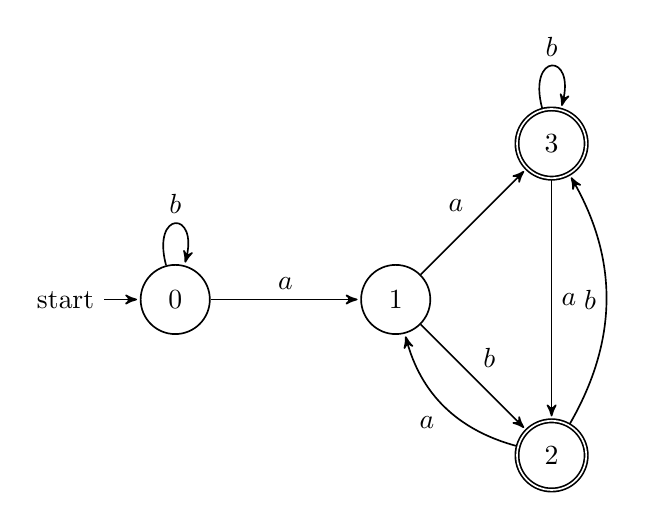
\begin{tikzpicture}[->,>=stealth',shorten >=1pt,auto,node distance=2.8cm,
                    semithick]
  \tikzstyle{every state}=[draw=black,text=black]

  \node[initial,state]            (A)                    {$0$};
  \node[state]                    (B) [right of=A]       {$1$};
  \node[accepting, state]         (C) [below right of=B] {$2$};
  \node[accepting, state]         (D) [above right of=B] {$3$};

  \path (A) edge [loop above] node {$b$} (A)
            edge              node {$a$} (B)
        (B) edge              node {$b$} (C)
            edge              node {$a$} (D)
        (C) edge [bend right] node {$b$} (D)
            edge [bend left]  node {$a$} (B)
        (D) edge [loop above] node {$b$} (D)
            edge              node {$a$} (C);
\end{tikzpicture}

\textbf{Answer:}

\begin{center}
\begin{tabular}{l}
\emph{T}(0, b) = 0, \\
\emph{T}(0, a) = \emph{T}(2, a) = 1, \\
\emph{T}(1, a) = \emph{T}(3, a) = 2, \\
\emph{T}(1, a) = \emph{T}(3, b) = \emph{T}(2, b) = 3, \\
where 0 is the start and both 2 and 3 are final states.
\end{tabular}
\end{center}

\begin{center}
\hspace{0.5cm}
\begin{tabular}{cc|cc}
           & $T$ & $a$ & $b$\\
     \cline{2-4}
     Start & $0$ & $1$ & $0$\\
           & $1$ & $3$ & $2$\\
           & $2$ & $1$ & $3$\\
    Final  & $3$ & $2$ & $3$\\
\end{tabular}
\end{center}

\textbf{Section 11.2, Exercise 2.c} Use your wits to construct a DFA for each of the following regular
expressions.\\
a + b*

\textbf{Answer:}

\begin{center}
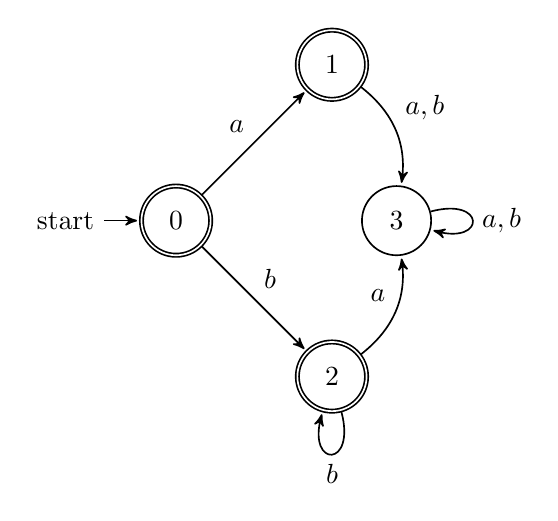
\begin{tikzpicture}[->,>=stealth',shorten >=1pt,auto,node distance=2.8cm,
                    semithick]
  \tikzstyle{every state}=[draw=black,text=black]

  \node[initial, accepting, state] (A)                    {$0$};
  \node[accepting, state]          (B) [above right of=A] {$1$};
  \node[accepting, state]          (C) [below right of=A] {$2$};
  \node[state]                     (D) [right of=A]       {$3$};

  \path (A) edge              node {$a$}   (B)
            edge              node {$b$}   (C)
        (B) edge [bend left]  node {$a,b$}   (D)
        (C) edge [loop below] node {$b$}   (C)
            edge [bend right] node {$a$}   (D)
        (D) edge [loop right] node {$a,b$} (D);
\end{tikzpicture}
\end{center}

\textbf{Section 11.2, Exercise 2.f} Use your wits to construct a DFA for each of the following regular
expressions.\\
a*bc* + ac

\textbf{Answer:}

\begin{center}
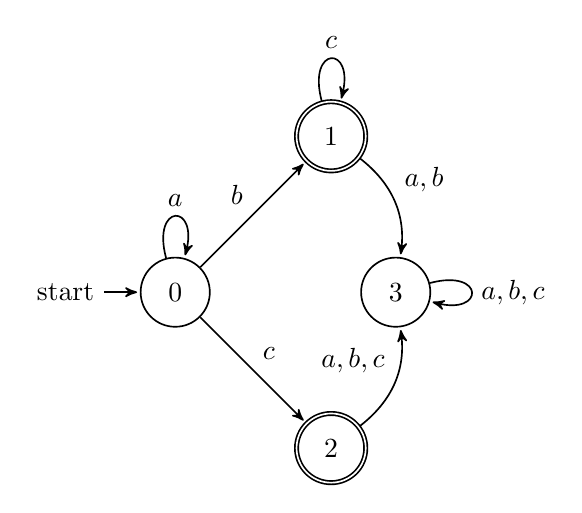
\begin{tikzpicture}[->,>=stealth',shorten >=1pt,auto,node distance=2.8cm,
                    semithick]
  \tikzstyle{every state}=[draw=black,text=black]

  \node[initial,state]            (A)                    {$0$};
  \node[accepting,state]          (B) [above right of=A] {$1$};
  \node[accepting, state]         (C) [below right of=A] {$2$};
  \node[state]                    (D) [right of=A]       {$3$};

  \path (A) edge [loop above] node {$a$}     (A)
            edge              node {$b$}     (B)
            edge              node {$c$}     (C)
        (B) edge [loop above] node {$c$}     (B)
            edge [bend left]  node {$a,b$} (D)
        (C) edge [bend right] node {$a,b,c$}   (D)
        (D) edge [loop right] node {$a,b,c$} (D);
\end{tikzpicture}
\end{center}

\textbf{Section 11.2, Exercise 4} Write down the transition function for the following NFA:

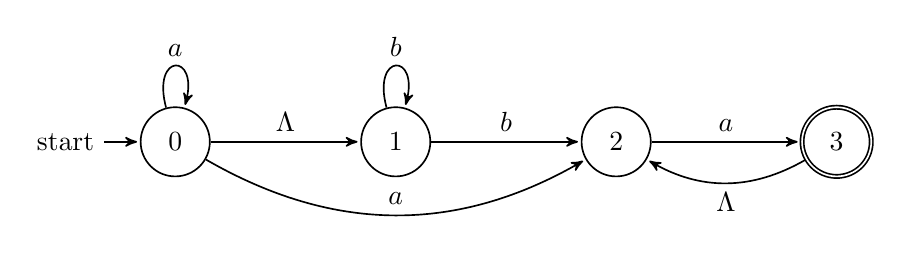
\begin{tikzpicture}[->,>=stealth',shorten >=1pt,auto,node distance=2.8cm,
                    semithick]
  \tikzstyle{every state}=[draw=black,text=black]

  \node[initial,state]   (A)               {$0$};
  \node[state]           (B) [right of=A]  {$1$};
  \node[state]           (C) [ right of=B] {$2$};
  \node[accepting,state] (D) [right of=C]  {$3$};

  \path (A) edge [loop above] node {$a$}       (A)
            edge              node {$\Lambda$} (B)
            edge [bend right] node {$a$}       (C)
        (B) edge [loop above] node {$b$}       (B)
            edge              node {$b$}       (C)
        (C) edge              node {$a$}       (D)
        (D) edge [bend left] node {$\Lambda$}  (C);
\end{tikzpicture}

\textbf{Answer:}

\begin{center}
\begin{tabular}{l}
\emph{T}(0, a) = 0, \\
\emph{T}(0, $\Lambda$) = \emph{T}(1, b) = 1, \\
\emph{T}(1, b) = \emph{T}(0, a) = \emph{T}(3, $\Lambda$) = 2, \\
\emph{T}(2, a) = 3, \\
where 0 is the start and 3 is final state.
\end{tabular}
\end{center}

\begin{center}
\hspace{0.5cm}
\begin{tabular}{cc|cc cc}
           & $T$ & $a$           & $b$           & $\Lambda$ \\
     \cline{2-5}
     Start & $0$ & $0$           & $\varnothing$ & $1$\\
           & $1$ & $\varnothing$ & $2$           & $\varnothing$\\
           & $2$ & $3$           & $\varnothing$ & $\varnothing$\\
    Final  & $3$ & $\varnothing$ & $\varnothing$ & $2$\\
\end{tabular}
\end{center}

\textbf{Section 11.2, Exercise 5,a} Use your wits to construct an NFA for each of the following regular
expressions. \\
a*bc* + ac

\textbf{Answer:}

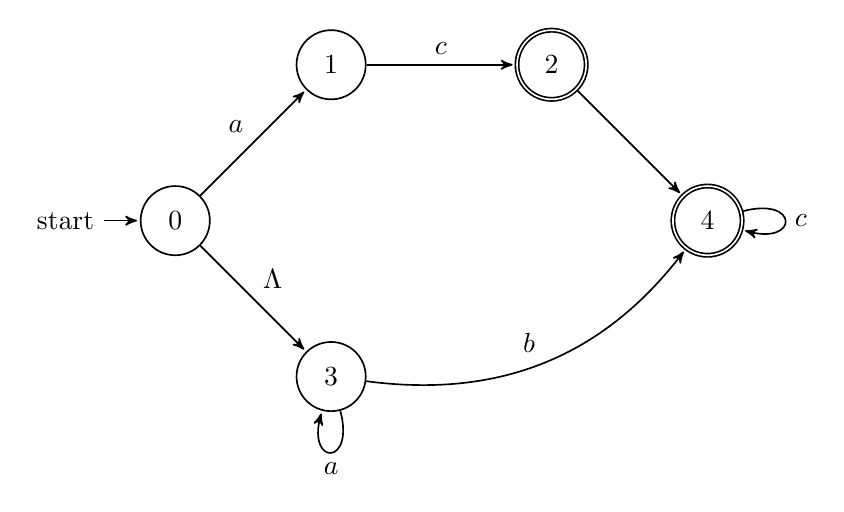
\begin{tikzpicture}[->,>=stealth',shorten >=1pt,auto,node distance=2.8cm,
                    semithick]
  \tikzstyle{every state}=[draw=black,text=black]

  \node[initial,state]   (A)                                                   {$0$};
  \node[state]           (B) [above right of=A]                                {$1$};
  \node[accepting,state] (C) [right of=B]                                      {$2$};
  \node[state]           (D) [below right of=A]                                {$3$};
  \node[accepting,state] (E) [below right of=A, above right of=D, right of=A]  {$4$};

  \path (A) edge              node {$a$}           (B)
            edge              node {$\Lambda$}     (D)
        (B) edge              node {$c$}           (C)
        (C) edge                                   (E)
        (D) edge [loop below] node {$a$}           (D)
            edge [bend right] node {$b$}           (E)
        (E) edge [loop right] node {$c$}           (E);
\end{tikzpicture}

\textbf{Section 11.2, Exercise 8,a} Given the following NFA:\\

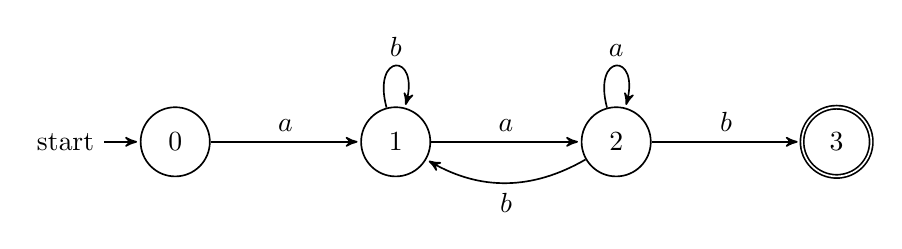
\begin{tikzpicture}[->,>=stealth',shorten >=1pt,auto,node distance=2.8cm,
                    semithick]
  \tikzstyle{every state}=[draw=black,text=black]

  \node[initial,state]   (A)               {$0$};
  \node[state]           (B) [right of=A]  {$1$};
  \node[state]           (C) [ right of=B] {$2$};
  \node[accepting,state] (D) [right of=C]  {$3$};

  \path (A) edge              node {$a$}       (B)
        (B) edge [loop above] node {$b$}       (B)
            edge              node {$a$}       (C)
        (C) edge [loop above] node {$a$}       (C) 
            edge              node {$b$}       (D)
            edge [bend left]  node {$b$}       (B);
\end{tikzpicture}

Use algorithm (11.2.4) to find two regular expressions for the language
accepted by the NFA as follows. \\
Delete state 1 before deleting state 2.

\textbf{Answer:}

\begin{align*}
new(0, 2) & = old(0,2) + old(0,1)old(1,1)^*old(1,2) \\
          & = \varnothing + ab^*a \\
          & = ab^*a, \\
new(2,2)  & = old(2,2) + old(2,1)old(1,1)^*old(1,2) \\
          & = a + bb^*a, \\
new(0,3)  & = old(0,3) + old(0,2)old(2,2)^*old(2,3) \\
          & = \varnothing + ab^*a(a + bb^*a)^*b \\
          & = ab^*a(a + bb^*a)^*b. \\
\end{align*}

\begin{center}
The final DFA is ab*a(a+bb*a)*b
\end{center}

\textbf{Section 11.2, Exercise 8.b} Given the following NFA:\\
Delete state 2 before deleting state 1.

\textbf{Answer:}

\begin{align*}
new(1, 3) & = old(1,3) + old(1,2)old(2,2)^*old(2,3) \\
          & = \varnothing + aa^*b \\
          & = aa^*b, \\
new(1,1)  & = old(1,1) + old(1,2)old(2,2)^*old(2,1) \\
          & = b + aa^*b, \\
new(0,3)  & = old(0,3) + old(0,1)old(1,1)^*old(1,3) \\
          & = \varnothing + a(b + aa^*b)^*aa^*b\\
          & = a(b + aa^*b)^*aa^*b.\\
\end{align*}

\begin{center}
The final DFA is a(b+aa*b)aa*b.
\end{center}

\end{document}